
\section{Narvis: System Design and Implementation}

% Thus, it has two kinds of users: editors, the data visualization experts who use Narvis to create an explanation slideshow, and audiences, the general audience who watch the slideshow created by ediors.

In this section, we first distill six design tasks based on our understanding of two kinds of end users, i.e., editors and general audience. Then, we describe the workflow of Narvis consisting of three phases (Figure \siwei{ref}), i.e., Automatic Analysis Phase, Human Editing Phase, and Viewing Phase.

% The workflow of Narvis includes three phases (Figure \siwei{ref}):  In Automatic Analysis Phase, the system accepts the input visualization, extracts graphical elements and classifies them into groups for further edit. 
% In Human Editing Phase, editors will be involved to modify the output from the Automatic Analysis Phase, and use the templates Narvis provide to craft a explanation slideshow. 
% In Reviewing Phase, audience can assess the slide show generated in Human Editing Phase. Their click activity and comments will be recorded and send to the editors, helping them improve the quality of the slide show. 

\begin{figure}
 \centering % avoid the use of \begin{center}...\end{center} and use \centering instead (more compact)
 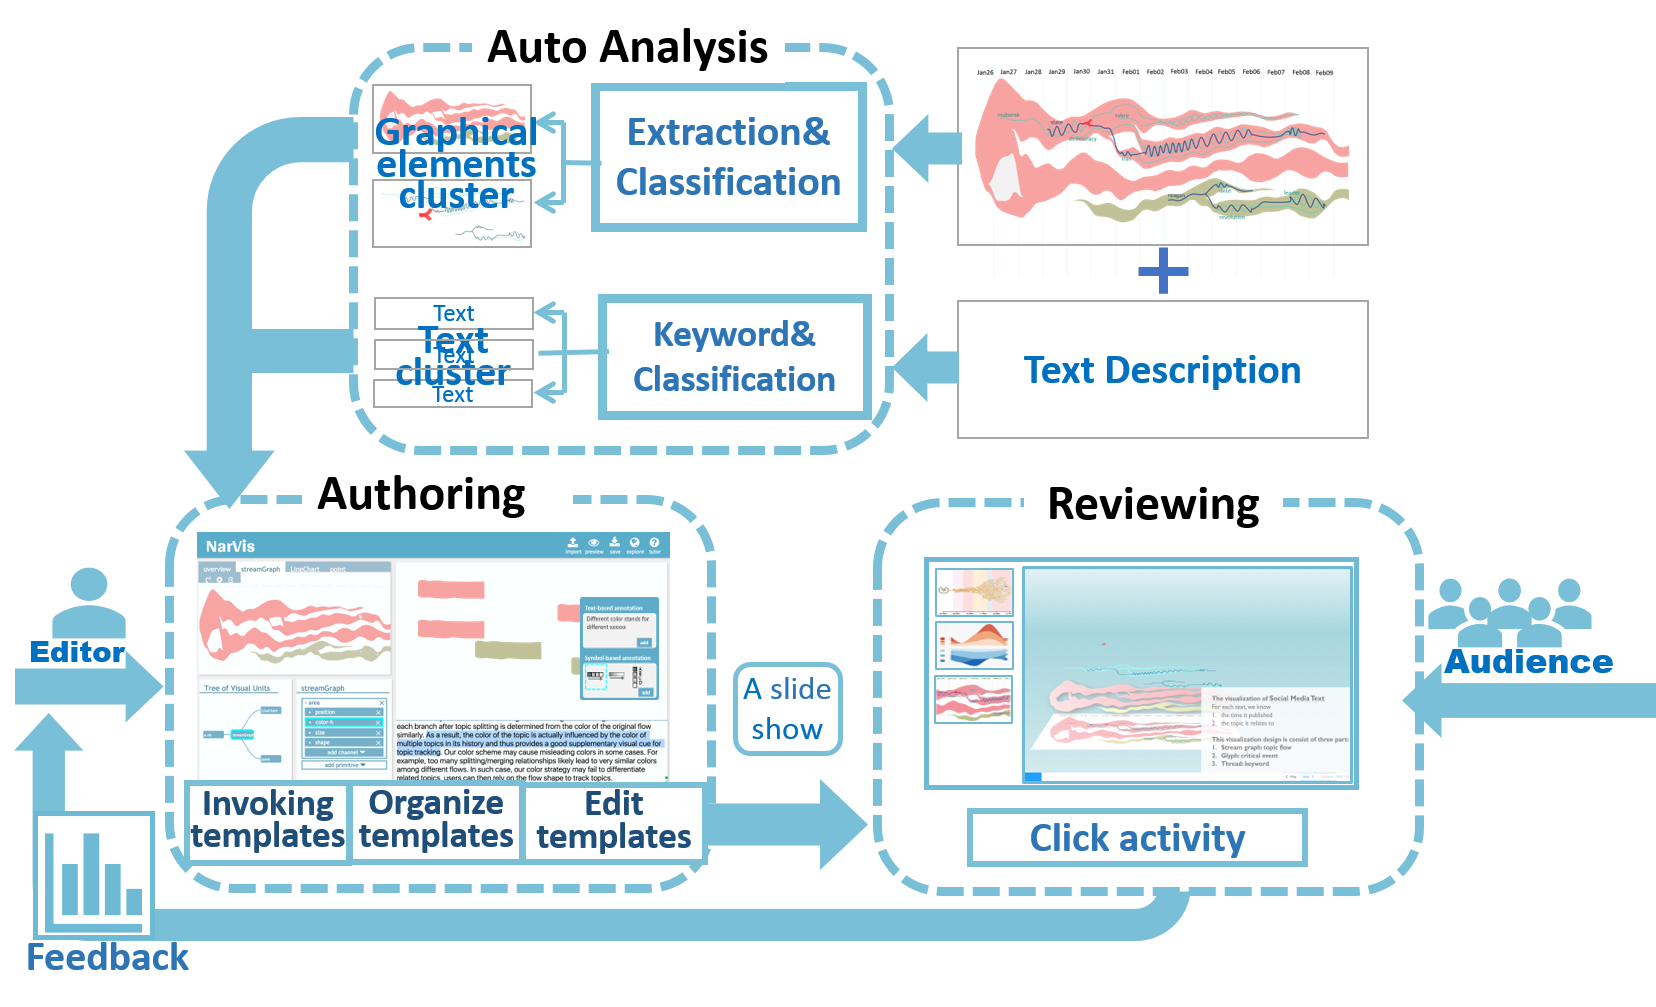
\includegraphics[width=\columnwidth]{overview}
 \caption{The system overview}
 \label{fig:overview}
\end{figure}

\subsection{User Perspectives and Methods}

Narvis aims to offer an efficient, expressive and friendly authoring tool for experts in data visualization, assisting them to create a slideshow to introduce advanced visual design to general audience.  
Hence, we identify two different user perspectives: the editors and the general audience perspectives. Editors are visualization experts who have the need to create a slideshow to communicate visual design. General audience have no prerequisite for visualization. They gain understanding of the visual design by watching the slideshow. 

To understand the current practice of making slideshows and the experience of reading tutorials, we collaborated with two teaching assistants (TAs) of a Data Visualization course and seven undergraduate students (UGs) taking this course. The two TAs are postgraduate students whose research interest is information visualization. Their duty of this course involves making slides for explaining visual design appears in major publications in the field of data visualization. The seven UGs have little background in visualization before the class, and have taken this course for less than one month.  

We began by conducting semi-structured interviews with TAs, whom we identified as editors, and UGs, who are general audience. During the interviews with TAs, we asked their workflows of making slideshows and explaining visual design. To identify opportunities for Narvis, we also asked them to enumerate a list of challenges faced in the workflows. In the interviews with UGs, we asked their comments in reading the slideshows and attending course lectures. Then, we used mind-mapping to find clusters in their comments that defined goals for an ideal slideshow. 


% two editors and seven general audience, respectively. Both interviews are semi-structured. 

% We should take editors and audiences alike into consideration for the design of Narvis. We conducted a interview with 3 experts in data visualization, asked what they could expect for an authoring tool for crafting an introduction slideshow. 
% We also constructed an interview with 7 undergraducate students. They have no prior experience in data visualization, and they just come back from a lecture about data visualization, which, as they said, ``totally confused'' them. They talked freely about what has confused them.
%It is interesting that there are some overlap between the requirements from editors and that from audience. For example, they both require slide  


% Based on this interview, as well as  our own experience and examination of literature, we settle on six design considerations(DCs) for the aspect of editors (DE) and that of audiences (DA). 

\subsection{Design Tasks}
Based on our observations and the interviews, we categorize six design tasks to guide the design of Narvis.


%Our premise is that the editor is familiar with a visualization design but unclear how to educate his audiences in an efficient way. Since the background of the audiences cannot be guaranteed, we assume they all have no prior knowledge in data visualization. 

\textbf{DE1. Efficiency}
There are many presentation tools, such as Power Point\footnote{https://office.live.com/start/PowerPoint.aspx}and KeyNote\footnote{http://www.apple.com/keynote/} that can be used for introducing a data visualization. But it can be time-consuming and tedious to use them for introducing a complex visualization, which has lots of graphical elements and various visual grammar.

\textbf{DE2. Support feedback.} ``When I present my design in public, I always wonder whether my audience get my idea. Do I explain too fast or too slow'', one participant said. Having access to the audience's feedback is crucial for the editors to improve  the quality of their introduction, making it more understandable and attractive.  
%We implement a click collector which will automatically record click activity when audience view the explanation in our system. The click stream data can reveal information about viewing order, for example, the audience might skip one slide or go back to revisit another, the time spent on each slide, the degree of understanding at each part.The audience can also write down their comments while reviewing such an introduction slide show. Editor can adjust the narrative sequence as well the level of details based on these feedbacks. 

\textbf{DA3. Control the density of information flow.} 
All interviwees mentioned that they experienced information overload during the lecture. Thus, they hope the introduction slideshow can well control the density of information flow, only revealing a proper amount of information at a time. 

\textbf{DA4. Avoid unconscious ignorance}

Experts in data visualization, prone to treat some visual encodings as evident, might unconsciously ignore some crucial information when introducing a visualization. However, for these with no prior knowledge about data visualization, the lack of such information can totally confuse them. 

\textbf{DA5. Clear structure.}

The complicated relationship, spatial and logical alike,  between different graphic elements is one of the biggest barriers that impedes a smooth communication of visual encoding scheme. 
%By encouraging users to refine the clusters of graphic elements, to figure out relationship between visual units by editing a unit tree, and to modify the narrative templates we offered, we aim at motivating users to sort out the structure of a visualization, which will then result in a better-organized narrative sequence. 


\textbf{DA6. Emphasis on conveying intuitive concepts.} 

 Although algorithm might be crucial for the achievement of a visualization design, some of the interviees show little interest in it. 
 
 %\textbf{DA7. Information repetion}
 %When introducing a visulization design, it is common for the audiences to forget previous information or lose the sense of overview. Information repetition, also called as redundancy, helps with visualization recall and understanding. \cite{borkin_what_2013}}
 %by providing simplified sentence pattern for annotation adding, we skip such parts in purpose.

%The audience of the generated narrative explanations are ordinal people, and they usually have no interests in understanding the algorithm employed in a visualization design. For example, the comprehension that a transition line indicates public attention shift from one topic to another is enough for them. Explicating how to quantify public attention shift only bores the audience, even scares them away.

\subsection{Phase1: Auto Analysis}\par
The auto analysis has two parts: one for input image and one for input text. It automatically extract the graphic elements and divide them into different cluster, facilitating later editing.(DE1) Note that the textual input is not necessary but it provides hints when editors add annotations manually in the Human Editing Phase.(DE1)
 \subsubsection{Analysis of input image}
The auto analysis of input image has three main steps. It first detects all primitives that it finds in the given image and also detects any labels that are present in the visualization. It will then cluster objects that are spacially linked and extract non-target objects. Finally, it will fill in any empty spaces left inside objects from extraction with the appropriate color so as to show the target object in its entirety.

The first step, object detection, is done by iterating through all the pixels on the bitmap. At every iteration, we first check to see if this pixel has already been tagged as part of an object. If not, we know that this pixel forms a part of a new object.We explore the colors of the neighboring pixels, where the neighbors are chosen such that the distance between the current pixel and a potential neighbor is less than 3. If the difference in color between a neighbor pixel and the current pixel is less than a threshhold, the neighboring pixel is tagged as part of the same object. Once all neighbors have been classified as either part of the same object or not, we choose another pixel that was classified as part of the same object and apply this algorithm again. This is a modified BFS algorithm and allows us to identify all unique ojects in the given visualization.

Once all the objects have been detected, we have to extract a target object. To extract an object means to only select the pixels that are classified as part of this object, so we should remove all objects that are not part of this object and we should extract objects that are inside our target object.It is trivial to set all pixels that are not within or part of our object to have color white. For objects that are inside our target object, i.e. those objects that are clustered with out target object, we will first detect that object then programmatically change its pixels to white.

Once we have completed extraction, we have the issue of these white spaces. The reason this is an issue is because an extracted object might have been dividing two objects, and so when it is extracted, we lose the boundary between our target object and another object, which can cause confusion as to whether that white space should be colored in or not. To solve this boundary problem, we create a queue of the white spaces, with each data point giving the starting and ending point of that space. We then look at the intervals between enclosed white spaced objects, if that interval is above a threshhold, we take that white space to not be part of our object. If it is below our threshhold, then we enclose the white space with the target objects color, creating a boundary for it. The main difference is that for objects not within our target object, we do not create a boundary, whereas objects within our target object are enclosed with the target objects color.\par
\subsubsection{Analysis of input textual description}
For the input textual description, we offer a basic text detection and classification algorithm, which uses a dictionary of terms that are highly correlated with certain channels. E.g. the word "length" is highly correlated with the size channel. To do the text detection, we first classify each sentence depending on whether it contains any of the key words in our dictionary. If it contains a key word for one of the channels, the sentence is tagged as being a description of that channels visualization. Once we have tagged all the sentences, whenever a channel is selected, we show the entire text that was inputted and highlight the text that has been tagged as descriptive of that channels visualization.

The algorithm we proposed is a compromise between efficiency and performance. At this time point, it is limited for image with high quality and clear edges, but its performance can be improved by applying a more advanced algorithm, such as the method based on patch detection and clustering mentioned in Revison\cite{savva_revision:_2011}.

\subsection{Phase2: Human Editing}
In Narvis, designers specify visualizations as a hierarchy of visual units with visual properties
\subsubsection{The interface for editing}
The interface of editing mode is composed of the following panels. We arrange the position of these panels and their content to better match the observed authoring work flow: refine clusters, bind with templates, organize the structure of visual units, modify templates, add annotation. 

\textbf{\textit{Source Panel}: extracting and organizing graphic elements}\par
FigSource is a tabbed panel where the extracted graphical elements are associated with different tabs based on the pre-cluster results. The user add, delete, modify the graphical elements associated with each tab, making sure that 1) All the graphical elements of the same visual unit is with one tab 2) every graphical element belongs to one and only one tab. For each tab, which actually equals to a visual unit now, the user call a template from our library in a drop-down list. 

\textbf{\textit{Tree Panel}: clarify the structure of a visualization}
\textit{Unit tree} panel tends to motivate the users to figure out the relationships between different visual units througn interacting.  
In the \textit{Unit Tree} panel, all visual units are shown as tree nodes.
With Interactions as simple as dragging and dropping, the users organized and display the structure of the visual units in the panel, like what we have discussed in section 3.3.(DA5) To help people better identify the relationship between visual units, which might be a new concept for them, we include a tutorial here. Even though learning the relationship between visual units requires extra effort and time, we believe it is worthwhile since it can give people a better understanding about the structure of a visualization. Based on the tree diagram, Narvis will refresh the narrative sequence of visual units. 

 \textbf{\textit{ Unit Panel \& Editor panel}: personalized modification}
 
 Narvis provides templates to achieve high efficiency, but it also allow the users high flexibity to modify these temples, thus guaranteeing the expressiveness of this system. 
 
Editors can edit a template in \textit{Unit Panle} by selecting a node on the \textit{Tree Panel}.For each visual units, the template enumerates possible encodings and leave the users to delete unemployed one, thus eliminating the unconscious missing of crucial information. (DA4)It also recommends a narrative sequence based on the metrics we mentioned in section 3.1.4. (DE1, DA3, DA5) 
 
In the editor panel, users get further to access the \textit{grammar} of each visual primitives, add a short annotation to describe it(DA6), refine or remove the animation we embedded in a template. 

\subsubsection{A library of templates}
We propose a library of templates for the narrative explanation of a visualization. A templates is a set of slides that tends to introduce a visual unit, which can be descibed as an orthogonal combination of a visual primitive and a construction rule, as shown in tab.1. Since advanced visualization design is the assembly of miscellaneous visual units, we conjecture such templates can achieve a high level of efficiency for the explanation of a viusalization. (DA1)Meanwhile, allowing users a high flexible, friendly interface to edit offered templates, Narvis maintains a considerable level of expressiveness and accessibility. 

\textbf{Types of templates}

The initial set of templates provided by Narvis can be described as  a 9*4 matrix, 9 types of visual primitives and 4 types of construction rules. Narvis is extensible, new templates can be added by its developer through programming, or by end users through uploading their modified templates. At the same time, all the supported templates are classified into a certain cell of the 9*4 matrix, so as to avoid overwhelming users with a cornucopia of confusing options.

\textbf{Templates design}

We apply the analysis and theory model in section 3 for the design of templates. A template has three components: 1) a well-considered narrative sequence for visual grammar explanation, which  is discussed in section 3.3 and reveal encoding grammar gradually(DA3); 2) Embedded a series of narrative techniques such as attention cues, animated transitions, information repetition, to orientate visual attention and facilitate perception; 3) Formatted sentence for annotations (DA6) that will be gradually disclosed in the slide show. (DA3)

With a visual unit, more specifically, a set of graphic elements, as input, a templates will generate a series of slide show and each slide is responsible for the explaining of one visual grammar. A visual properity show on a slide only after its grammar has been explained. For example, if we havn't explain the encoding of color, all the object in current slides will be gray. These slides are sorted based on the narrative sequence we discussed in section 3.3. The graphical elements in different slides, which might have different visual appearance, are perceptively connected through morphing animation.

\textbf{Animation embedded in templates }

Narvis provides 8 types of animation, implement them in templates based on their effects on human attention and perception(DA1), which has been widely discussed in previous work.\cite{robertson_effectiveness_2008, waldner_attractive_2014, heer_animated_2007}We also provide an novel decomposition animation at the beginning of the introduction slide show to engage the audience as well as to help them get a sense of overview.

\begin{table}[tb]
  \caption{A summary of animation provided}
  \label{tab:animation}
  \small
  \centering
  \begin{tabular}{p{1cm}|p{0.9cm}|p{0.9cm}|p{0.9cm}|p{1.5cm}|p{0.9cm}}
  \toprule
 \textbf{Animation} &\textbf{Engaging} & \textbf{orientate attention} & \textbf{perception} &\textbf{working scenario} &\textbf{ref} \\ 
  \midrule
  \textbf{Morphing} &\checkmark & \checkmark &\checkmark & grammar of size, grammar of shape & \cite{ruchikachorn_learning_2015} \\ 
  \midrule
  \textbf{Blur} &   &\checkmark  &   & focus+context & \\ 
  \midrule
  \textbf{Flicker} & & \checkmark &  & focus & \\
  \midrule
  \textbf{Motion} & \checkmark & \checkmark & \checkmark &grammar of position &  \\
  \midrule
  \textbf{Zoom-in/out} & \checkmark &\checkmark &  & focus&  \\
  \midrule
  \textbf{Annotation} &  & \checkmark &\checkmark &   textual explain & \\
  \midrule
  \textbf{Fade in/out} &  & \checkmark &  & & \\
  \midrule
  \textbf{Decompose} & \checkmark &  &\checkmark & Show how a visualization is composed by visual units & A novel design bu us \\
  \bottomrule

  \end{tabular}
  \vspace{1mm}
\end{table}


Animation is a double-edge sword, which introduces both benefits and pitfalls. We are not discussing the effects of animation here. Editors can choose to remove these animation if they prefer an abstract slide show or they are suspicious of the effects of animation. 


\subsection{Phase3: Viewing}
\subsubsection{The interface for audience}
The interface of audience is composed of two panels.

\textbf{\textit{Gallery:}the collection of generated slide show}
 
Gallery exhibit all the slide show produced by editors and saved in Narvis. Every slide show is presented by a image, the visualization it tends to explain. By clicking on the image, users can watch this slide show in the \textit{Screen} panel. 

\textbf{\textit{Screen:}  review and comment}
Every slide show displayed in \textit{Gallery}is a series of slides, each of which is responsible for the delivery of one simple encoding information, for example, the horizontal position indicates time. In the \textit{Screen} panel, users click buttons to move forward or backward to view these slides. 
\subsubsection{Generated Report}
The report visualize the click activity of audience in the form of a stacked bar chart. The heigh of the bar indicates the time spent on watching this slide. If audiences go back to revist a slide while viewing, a bar will be stacked on the top of previous one. If there are animation in the slide show, a white line will be drawn on the bar chart, indicating the animation playing time of each slide, thus can indicate whether an animation is too fast or too slow. (DE2)
\subsection{A working scenario}
Jessica has extensive experience in the field of data visualization, and has implement a visual analytics tool in a review service website based on the design of OpinionSeer\cite{wu_opinionseer:_2010}. To help audience better understand this design, she needs to publish a tutorial accompanied with it.
% Here, we demonstrate the utility of Narvis through the creation of a narrative explanation of a visualization design that published in TVCG (http://ieeexplore.ieee.org/stamp/stamp.jsp?arnumber=5613449). 

% \subsubsection{Motivation}Jessica, a expert in data visualization, realizes the promising prospect of implementing this visualization design in an on-line review service website like Yelp. (pg student to classmates? prof to a journalist? prof with collaborators from other fields?  )\par
% However, she has to present this design in a general meeting to get the financial support. She is familiar with this visualization design, yet not sure whether her audiences, with little knowledge about data visualization, can quickly learn this visualization design from her introduction. Without clear awareness of the visual encodings, audience can hardly identify the interesting patterns this visualization reveals and realize its utility.  
% A traditional way is to add highlights and annotations in the original visualization. But Jessica worries about the effectiveness of information delivery. 
% She considers about applying "focus + context" techniques,  but it will introduce some complicated operations for her, who has no experience in image editing. 
% Moreover, with the large number of visual encodings existing, she fails to determine an optimized order for explaining them. Even though she has many years of experience in data visualization, she never think about this issue before. 
% She then turns to Narvis for help. 

% She first imports visualization design, in the form of a PNG file, and the corresponding text description, which she directly copy from the paper, into the system. 
First, she loads the screen-shot of her system, as well as a piece of textual description, into Narvis.
% After a few seconds, the system automatically detects graphics elements with a edge detection algorithm and cluster them based on their features. The algorithm cannot be perfect. For example, it puts geo ring and calendar ring in the same cluster based on their similar appearance. 
After a few seconds, the system automatically extracts the graphics elements and clusters them based on features. As Figure\siwei{ref} shows, Jessica obtains four clusters. 

Then, she defines visual units based on clusters. By default, each cluster includes all graphics elements belonging to one visual unit. However, she observes that geographic ring and calendar ring are in the same cluster due to their similar appearance. Therefore, she divides it into two clusters, containing geographic ring and calendar ring respectively.
% then refines the clustering results, making sure every graphic elements in one visual unit is put in one cluster \textbf{figure xxx}. Finally she obtains four clusters.

Next, she chooses narrative templates for each visual unit. 
%Some visual units, such as the triangle scatter plot, are novel and no narrative template in the library is able to match. Therefore, Jessica chooses the template of regular scatter plot for best match.
% for triangle scatter plot, which differs from the triangle plot in the encoding of position. 
Moreover, Jessica edits the narrative templates based on her design. 
% In the templates, we enumerate all the possible visual encodings. 
She goes through all four templates in the ``\siwei{what is in-unit}in-unit'', and deletes the visual channels with no encodings, such as \siwei{sth}. 
Through drag and drop, Jessica further organizes the structure of the unit tree based on the relationships between units. For example, \siwei{some example}

Jessica further improves the quality of animation by adding annotations and strengthening the binding between data and graphic elements. 
% When adding annotation to a certain channel, the related text will highlight in the text area, aiming to offer a better user experience.   


To refine the readability of the tutorial, Jessica asks several friends, who have no experience in data visualization, to watch the tutorial before release. Narvis collects their viewing behavior from click activities, generates statistics results, and visualize it in the form of stacked bar chart , which helps Jessica answer questions like \textit{``which slides do they skip?''}, \textit{``which slides do they review several times?''}, and \textit{``which slides do they stay for a long time?''}.
% These click sequence data provides cues for Jessica to strengthen and refine the readability of the tutorial. 

% revealing information such as, ,   



